\documentclass[10pt,serif,t]{beamer}

\usepackage[section]{placeins}
\usepackage[style=numeric-comp,natbib=true]{biblatex}
\usepackage{minted}
\usepackage{amsmath,mathtools}

\addbibresource{DanNixon_ProjectPresentation.bib}

\usepackage{graphicx}
\DeclareGraphicsRule{*}{mps}{*}{}

\newcommand\Heading[1]{%
  {\bfseries#1}\par\smallskip}

% Environment for a slide
\newenvironment{Slide}[1]
{
\begin{frame}[fragile,environment=Slide]
  \frametitle{#1}
  \section{#1}
}
{
\end{frame}
}

% Environment for a sub slide
\newenvironment{SubSlide}[1]
{
\begin{frame}[fragile,encirclement=SubSlide]
  \frametitle{#1}
  \subsection{#1}
}
{
\end{frame}
}

% Environment for a sub sub slide
\newenvironment{SubSubSlide}[1]
{
\begin{frame}[fragile,environment=SubSubSlide]
  \frametitle{#1}
  \subsubsection{#1}
}
{
\end{frame}
}

\title{The Application of Robust Analysis Methods on Sparse Data for
       Mass-Resolved Neutron Spectroscopy}
\author{Daniel Nixon \\
        (Supervisor: Dr Paolo Zuliani)}
\date{November 2015}

\begin{document}

\frame{\titlepage}

\begin{Slide}{Project}
  \Heading{Aim}
  To improve the data analysis routines for mass selective neutron spectroscopy
  (MANSE) on the VESUVIO instrument at the ISIS facility, Rutherford Appleton
  Laboratory, Oxford, UK.

  \par\bigskip
  \Heading{Objectives}
  \begin{itemize}
    \item Development of robust variance/covariance analysis routines for
          relevant models describing MANSE data
    \item Extension of the analysis routines to use Bayesian methods to
          determine likelihood of masses or responses in a model
    \item Evaluate the effectiveness of the developed routines through the use
          of case studies on well known samples
  \end{itemize}
\end{Slide}

\begin{Slide}{The ISIS facility}
  \begin{columns}[T]
    \begin{column}{.55\textwidth}
      \begin{figure}[h!]
        \centering
        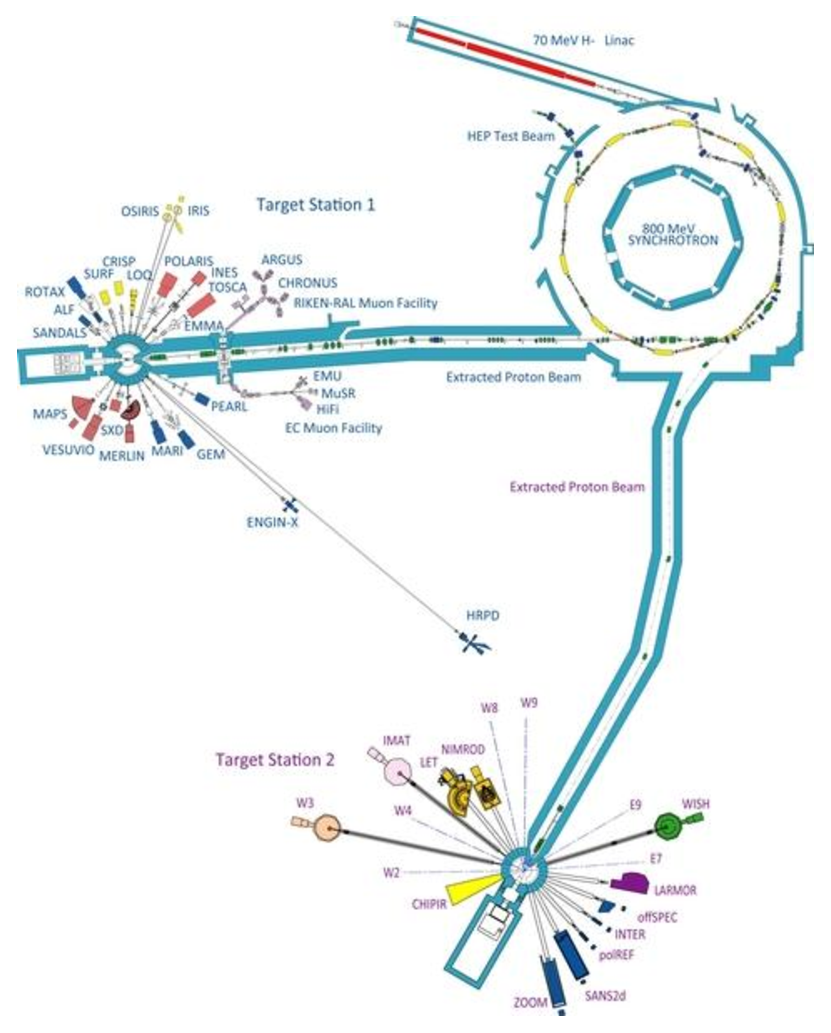
\includegraphics[width=0.9\textwidth]{graphics/isis_diagram.eps}
        \caption{ISIS layout \cite{isis_website}}
        \label{fig:isis_diagram}
      \end{figure}
    \end{column}
    \hfill
    \begin{column}{.44\textwidth}
      \begin{itemize}
        \item 70 MeV $\mathrm{H}^{-}$ linear accelerator
        \item 800 MeV 163m proton synchrotron
        \item TS1 receives 40Hz beam @ ~160$\mathrm{\mu Ah}$
        \item Neutrons produces when proton beam collides with Tungsten target
      \end{itemize}
    \end{column}
  \end{columns}
\end{Slide}

\begin{Slide}{The VESUVIO instrument}
  \begin{columns}[T]
    \begin{column}{.55\textwidth}
      \begin{figure}[h!]
        \centering
        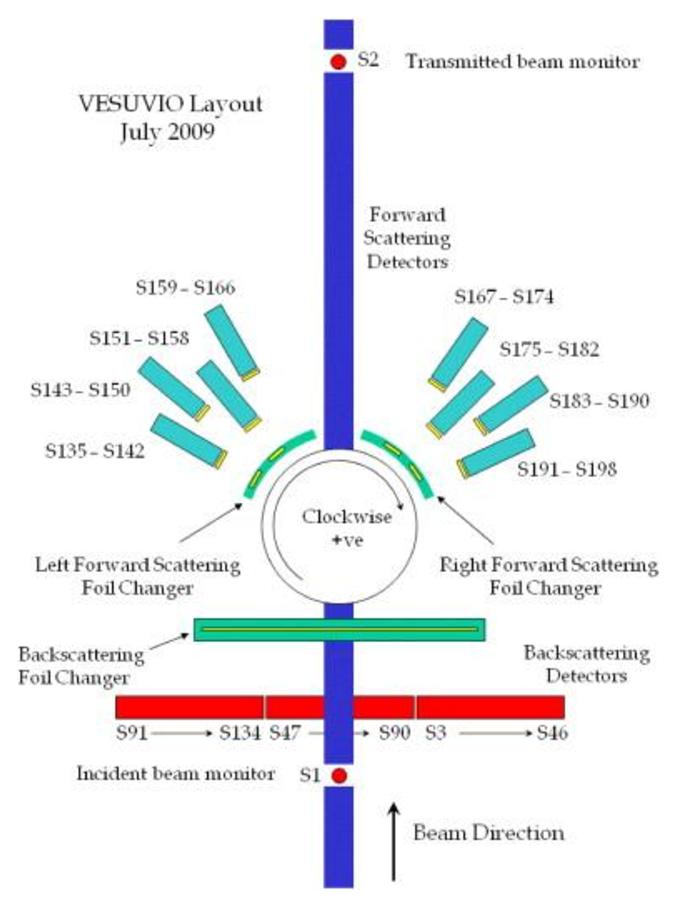
\includegraphics[width=0.8\textwidth]{graphics/evs_layout_july2009.eps}
        \caption{VESUVIO instrument layout \cite{calibration_of_evs}}
        \label{fig:vesuvio_layout}
      \end{figure}
    \end{column}
    \hfill
    \begin{column}{.44\textwidth}
      \begin{itemize}
        \item Neutron spectrometer and diffractometer (5-150eV)
        \item 64 yttrium aluminium perovskite (YAP) $\gamma$-ray detectors in
              forward scattering
        \item YAP detectors detect $\gamma$-rays emitted from gold foils when
              neutrons are absorbed
        \item 132 $\prescript{6}{}{\mathrm{Li}}$ doped neutron detectors in back
              scattering
      \end{itemize}
    \end{column}
  \end{columns}
\end{Slide}

\begin{Slide}{Current analysis workflow}
  \begin{columns}[T]
    \begin{column}{.55\textwidth}
      \begin{figure}[h!]
        \centering
        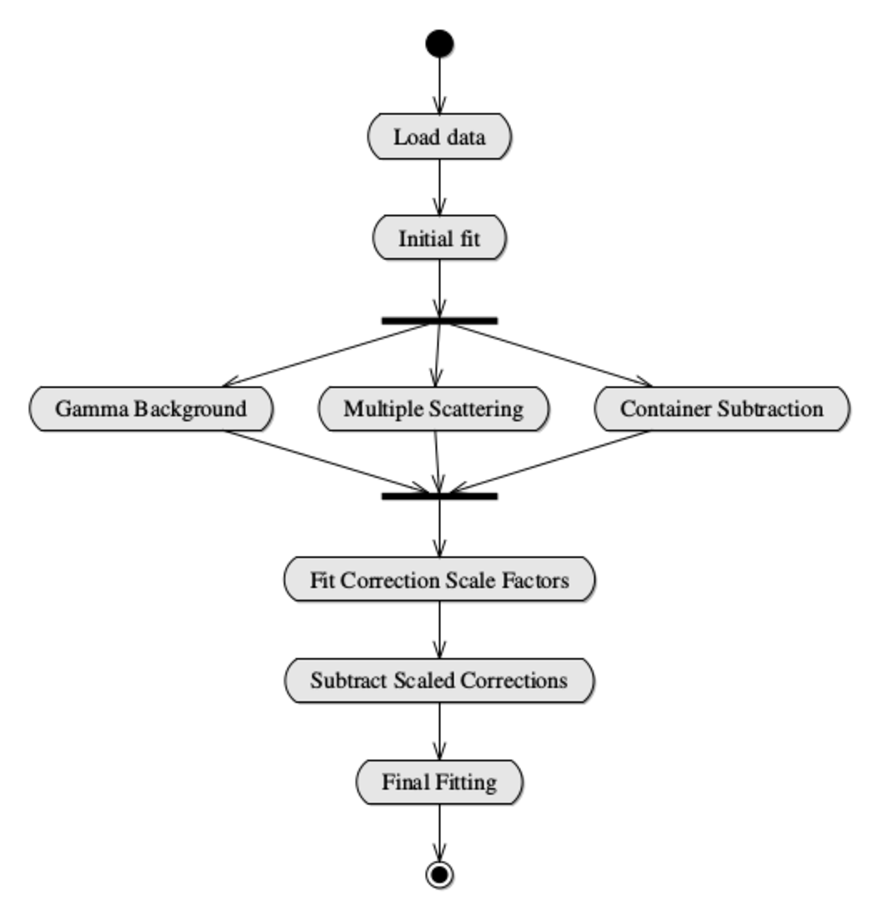
\includegraphics[width=\textwidth]{graphics/current_workflow.eps}
        \caption{Current data treatment workflow \cite{ral_tr_2015_007}}
        \label{fig:current_workflow}
      \end{figure}
    \end{column}
    \hfill
    \begin{column}{.44\textwidth}
      \begin{itemize}
        \item Implemented in the MANTID \cite{mantid} toolkit
        \item Set up using an approx. 80 line configuration script
        \item Assumes Gaussian distributions for mass profiles
        \item Requires prior knowledge of the sample composition
      \end{itemize}
    \end{column}
  \end{columns}
\end{Slide}

\begin{Slide}{Current analysis workflow - results}
  \inputminted[frame=lines,fontsize=\tiny]{python}{listings/tof_fit_extracts.py}
  \begin{figure}[h!]
    \centering
    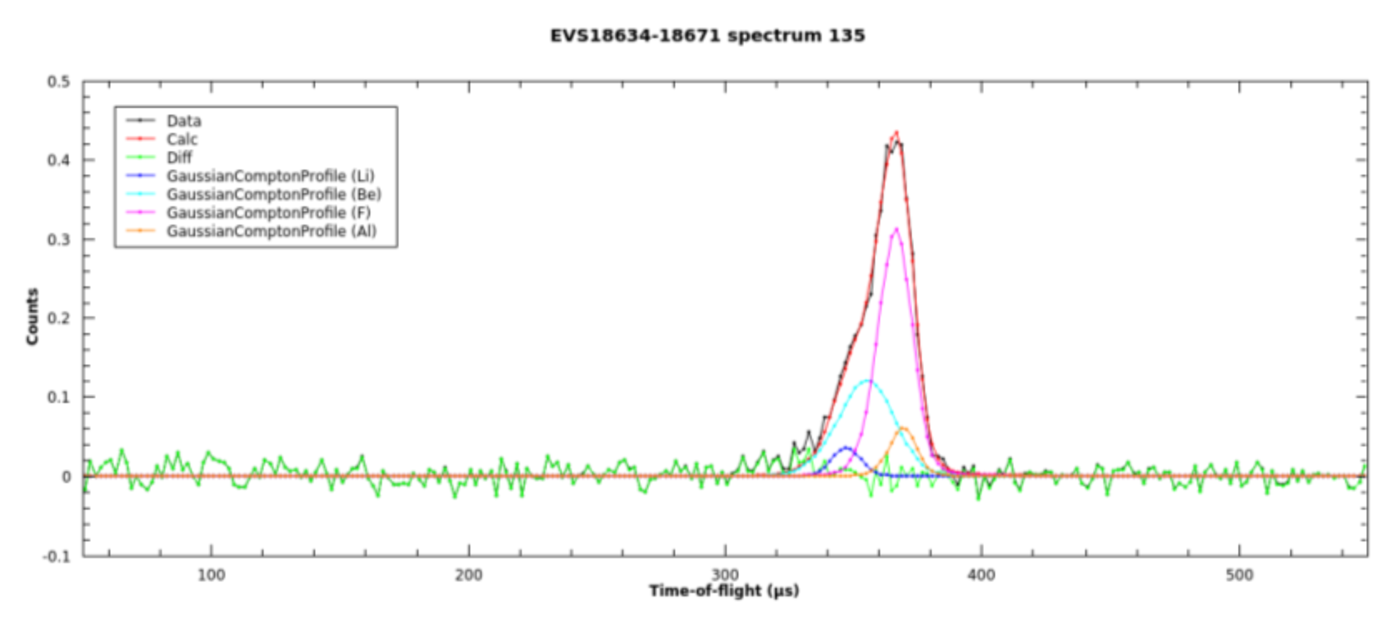
\includegraphics[width=0.8\textwidth]{graphics/current_workflow_fitting.eps}
    \caption{Fitted results \cite{ral_tr_2015_007}}
    \label{fig:current_workflow_fitting}
  \end{figure}
\end{Slide}

\begin{Slide}{Technologies}
  \begin{columns}[T]
    \begin{column}{.55\textwidth}
      \begin{figure}[h!]
        \centering
        \includegraphics[height=0.5\textheight]{out/mantid_algorithms.1}
        \caption{MANTID algorithms}
        \label{fig:mantid_algorithms}
      \end{figure}
    \end{column}
    \hfill
    \begin{column}{.44\textwidth}
      \Heading{MANTID framework}
      \begin{itemize}
        \item Cross platform neutron and muon data analysis package
        \item Used by neutron facilities throughout the world
        \item C++, Python, (Fortran)
        \item Main concepts:
          \begin{itemize}
            \item Workspaces
            \item Algorithms
            \item Curve fitting
          \end{itemize}
      \end{itemize}
    \end{column}
  \end{columns}
\end{Slide}

\begin{Slide}{Technologies}
  \begin{columns}[T]
    \begin{column}{.55\textwidth}
      \begin{figure}[h!]
        \centering
        \includegraphics[height=0.5\textheight]{out/mantid_fitting.1}
        \caption{MANTID fitting}
        \label{fig:fitting_workflow}
      \end{figure}
    \end{column}
    \hfill
    \begin{column}{.44\textwidth}
      \Heading{MANTID curve fitting}
      \begin{itemize}
        \item MANTID fitting framework
          \begin{itemize}
            \item Optimisation algorithms
            \item Fit functions
            \item Minimisers
            \item Cost functions (least squares)
          \end{itemize}
      \end{itemize}
      \Heading{3rd party libraries}
      \begin{itemize}
        \item GNU Scientific Library
        \item (SciPy, NumPy)
      \end{itemize}
    \end{column}
  \end{columns}
\end{Slide}

\begin{Slide}{Research/Planning}
  \begin{itemize}
    \item Determine relevant models for MANSE data and obtain papers detailing
          their mathematical definition
          \smallskip
    \item Obtain test data (experimental or simulated) containing a known sample
          for each model to be used for automated testing
          \smallskip
    \item Produce mock/proof of concept implementations of fitting algorithms
          for certain models (if required)
          \smallskip
    \item Alleviate any existing issues in the MANTID framework that may cause
          issues later in the project
          \smallskip
          \begin{itemize}
            \item e.g. issues with the FABADA minimiser
          \end{itemize}
  \end{itemize}
\end{Slide}

\begin{Slide}{Implementation Plan}
  \Heading{Phase 1 - MANSE fitting routines}
  By March 2016.
  \smallskip
  \begin{itemize}
    \item Development of new curve fitting routines, implemented within the MANTID framework
      \begin{itemize}
        \item knowledge of sample composition still required
      \end{itemize}
    \item Benchmarking the developed routines against VESUVIO data with well
          known samples
  \end{itemize}

  \par\bigskip
  \Heading{Phase 2- Bayesian analysis}
  By April 2016.
  \smallskip
  \begin{itemize}
    \item Removes the requirement for the sample composition to be known when
          using fitting routines developed in phase 1
    \item Allow use of FABADA \cite{fabada} (already implemented within MANTID)
          with analysis routines
  \end{itemize}

  \par\bigskip
  Ongoing unit and integration testing as routines are implemented.
\end{Slide}

\begin{Slide}{Implementation Plan}
  \Heading{Phase 3/Ongoing - Case studies}
  By May 2016.
  \smallskip
  \begin{itemize}
    \item Bayesian analysis of MANSE models in the presence of unwanted $\gamma$
          resonances
    \item Identification of components in VESUVIO spectra due to
          non-Gaussian distributions
    \item Kinetics of slow chemical or physical reactions
    \item Samples with unknown compositions, identification of trace
          elements/impurities (augmented by diffraction where appropriate)
  \end{itemize}

  \par\bigskip
  \Heading{Deliverables}
  Documentation of:
  \begin{itemize}
    \item routines implemented
    \item models they are used to fit
    \item critical analysis of their performance
  \end{itemize}
\end{Slide}

\begin{Slide}{References}
  \nocite{vesuvio_evs_mayers2012}
  \setbeamertemplate{bibliography item}{\insertbiblabel}
  \printbibliography
\end{Slide}

\end{document}
